\section{Project Plan}

\begin{frame}
	{Slides}

	\begin{itemize}
		\item
			Download the slides for local reference
		\item
			\url{https://cm.e-ale.org/2019/ELCE2019/iioinput/iioinput-elce2019-SLIDES.pdf}
	\end{itemize}
\end{frame}

\begin{frame}
	{What To Do?}

	\begin{itemize}
		\item
			The TechLab Cape has an accelerometer and a couple buttons.
		\item
			We'll learn how to read the position of the accelerometer axes.
		\item
			We'll also learn how to read the state of the buttons
		\item
			With that data, we have the foundation for a joystick driver.
	\end{itemize}

	     \begin{figure}[H]
		     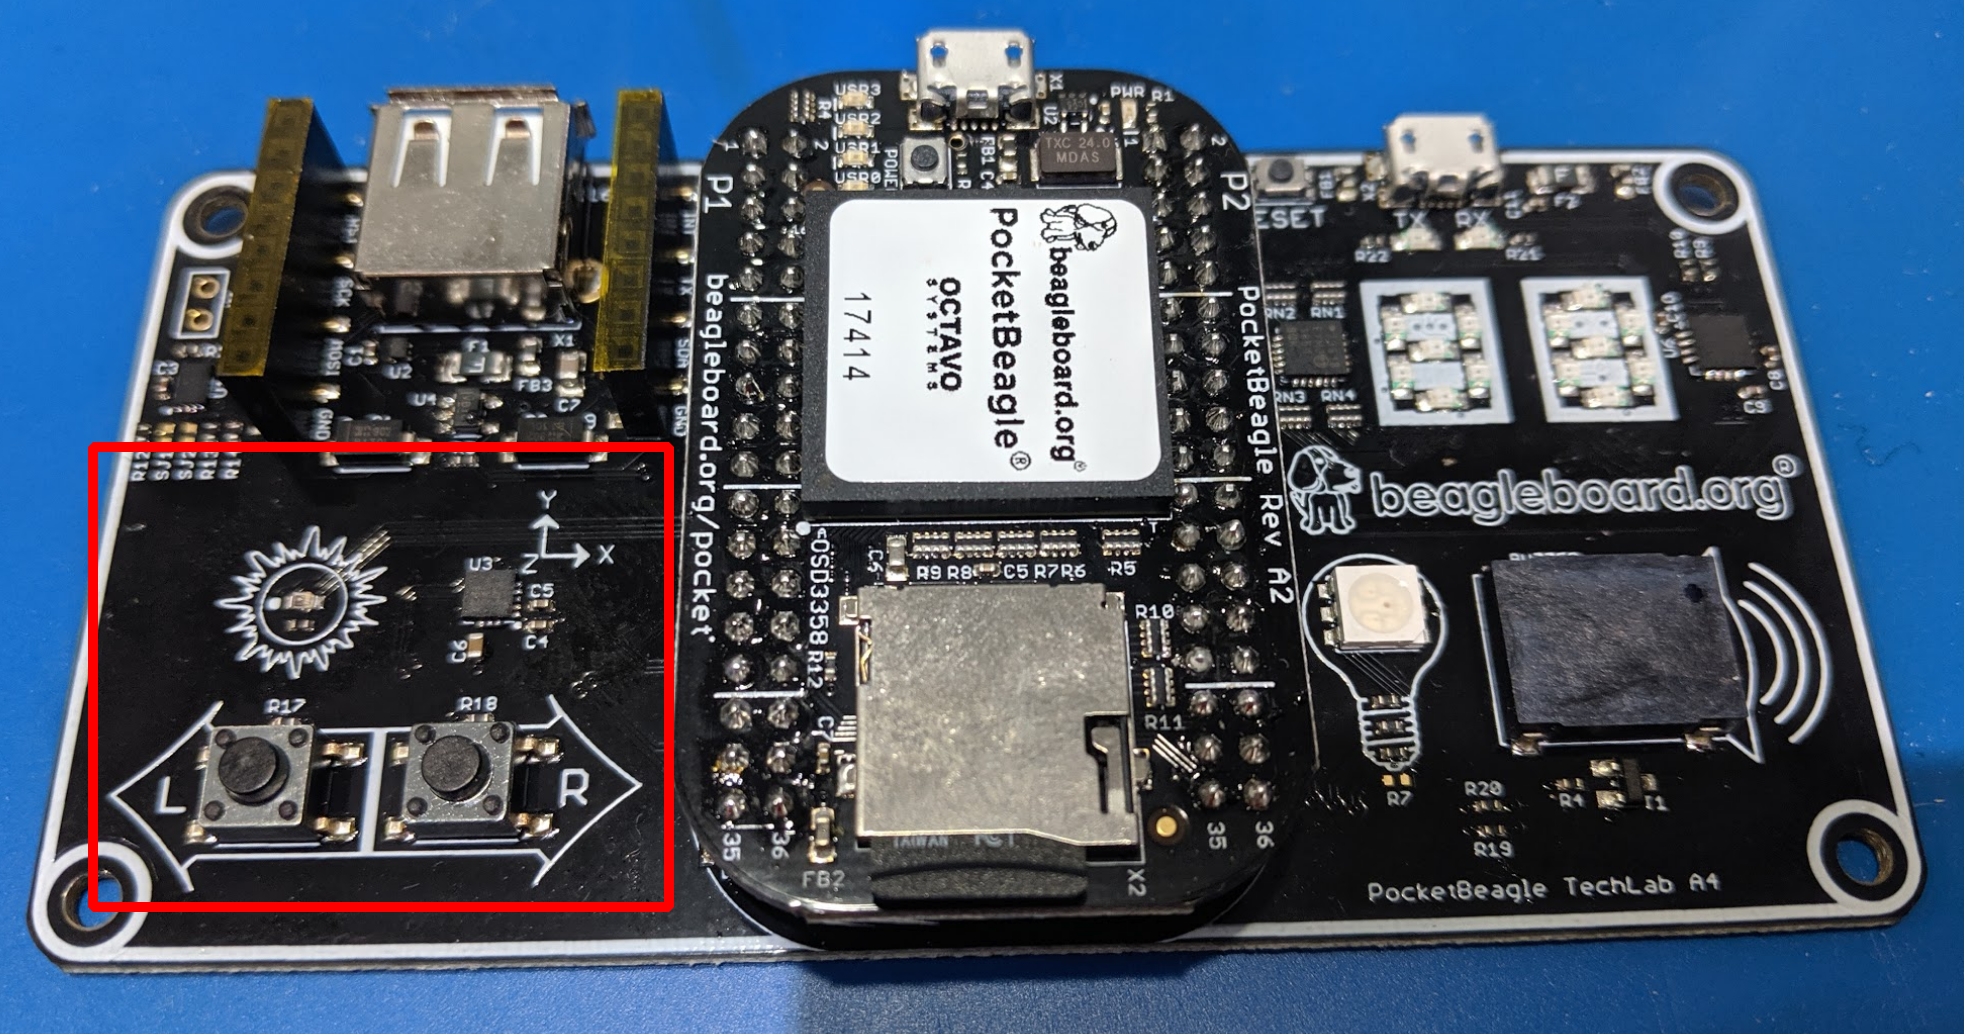
\includegraphics[width=3in]{IMAGES/techlab-annotated}
				       \caption{TechLab Cape}
	     \end{figure}
\end{frame}


\begin{frame}
	{Exact Steps}
	\begin{itemize}
		\item
			Understand how the accelerometer and buttons are interfaced in hardware
		\item
			Understand IIO and its purpose in the universe
		\item
			Learn how IIO exposes the accelerometer to the kernel and userspace
		\item
			Learn how to use libiio for userspace IIO interaction
		\item
			Write a accelerometer-based joystick driver and test it
	\end{itemize}
\end{frame}
